\documentclass{ximera}  

\title{The Dot Product}  

\begin{document}  
\begin{abstract}  
%abstract
\end{abstract}  
\maketitle 

In this section we review the dot product on vectors. This also includes the angle between vectors and the projection of one vector onto another.

\section{The Dot Product}

We begin with the definition of the dot product.

\begin{definition}
The \emph{dot product} of two vectors $\vec{v} = (v_1,v_2,...,v_n)$ and $\vec{w} = (w_1,w_2,...,w_n)$ in $\mathbb{R}^n$ is
\[
\vec{v}\cdot\vec{w} = v_1w_1+v_2w_2+\cdots + v_nw_n.
\]
\end{definition}

Notice that the dot product takes two vectors and outputs a scalar.

\begin{example}
$(1,6)\cdot (-3,-6) = -3-36=-39$

$(1,2,3)\cdot (7,-2,4) = 7-4+12=15$

$(1,7,-3)\cdot (3,0,1) = 3+0-3=0$
\end{example}

We can also compute the dot product using the magnitude (or length) of the vectors and the angle in between them.

\begin{proposition}
If $\vec{v}$ and $\vec{w}$ are vectors in $\mathbb{R}^n$, then
\[
\vec{v}\cdot\vec{w} = \|\vec{v}\|\,\|\vec{w}\|\cos\theta,
\]
where $\|\vec{v}\|$ and $\|\vec{w}\|$ are the lengths of the vectors $\vec{v}$ and $\vec{w}$, respectively, and $\theta$ is the angle between $\vec{v}$ and $\vec{w}$.
\end{proposition}

This is illustrated in the picture below.

\begin{image}
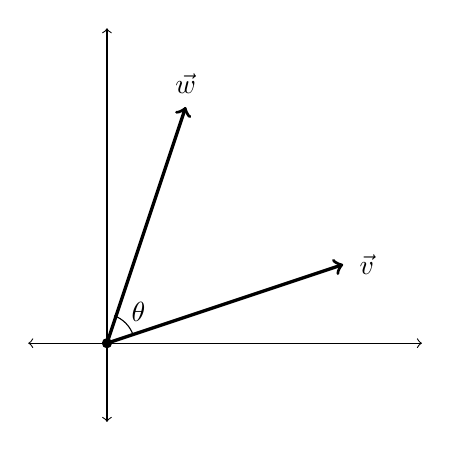
\begin{tikzpicture}
\draw[<->] (-1,0) -- (4,0);
\draw[<->] (0,-1) -- (0,4);

\node[draw, circle, thick, fill=black, minimum size=1mm, inner sep=0] at (0,0) {};
\draw[->, very thick] (0,0) -- (1,3);
\draw[->,very thick] (0,0) -- (3,1);
\draw (0.33,0.11) arc (20:70:.4);
\node at (.4,.4) {$\theta$};
\node at (3.3,1) {$\vec{v}$};
\node at (1,3.3) {$\vec{w}$};

\end{tikzpicture}
\end{image}

This provides us with a geometric interpretation of the dot product: it gives us a measure of ``how much'' in the same direction two vectors are (taking their lengths into account). This also gives us a useful way to compute the angle between two vectors.

\begin{example}
Consider the vectors $(1,4)$ and $(-2,2)$. We have
\begin{align*}
(1,4)\cdot (-2,2) &= -2+8= 6,\\
\|(1,4)\| &= \sqrt{1^2+4^2} = \sqrt{17},\\
\|(-2,2)\| &= \sqrt{(-2)^2+2^2}=\sqrt{8}.
\end{align*}
From $\vec{v}\cdot\vec{w} = \|\vec{v}\|\,\|\vec{w}\|\cos\theta$, we then have
\[
6 = \sqrt{17}\sqrt{8}\cos\theta.
\]
Solving for $\theta$, we obtain the angle between the vectors as
\[
\theta = \arccos\left(\frac{6}{\sqrt{17}\sqrt{8}}\right)\approx 59.04^\circ
\]
\end{example}

Furthermore, note that for nonzero vectors $\vec{v}$ and $\vec{w}$ in $\mathbb{R}^n$, their dot product is $0$ if and only if $\cos(\theta) = 0$. This means that $\theta$ would have to be $90^\circ$ or $270^\circ$, meaning that $\vec{v}$ and $\vec{w}$ are perpendicular. 

\begin{proposition}
Two nonzero vectors $\vec{v}$ in $\vec{w}$ in $\mathbb{R}^n$ are perpendicular if and only if $\vec{v}\cdot\vec{w} = 0$.
\end{proposition}

This provides us with a very useful algebraic method for determining if two vectors are perpendicular.

\begin{example}
The vectors $(1,7,-3)$ and $(3,0,1)$ in $\mathbb{R}^3$ are perpendicular, since
\[
(1,7,-3)\cdot (3,0,1) = 3+0-3=0.
\]
\end{example}

\section{Projection of one vector onto another}

We can also use the dot product to define the projection of one vector onto another.

\begin{definition}
For vectors $\vec{a}$ and $\vec{b}$ in $\mathbb{R}^n$, we define the \emph{vector projection} of $\vec{a}$ onto $\vec{b}$ as
\[
\textrm{proj}_{\vec{b}}(\vec{a}) = \frac{\vec{a}\cdot\vec{b}}{\|\vec{b}\|^2}\vec{b}  = \frac{\vec{a}\cdot\vec{b}}{\vec{b}\cdot\vec{b}}\vec{b}.
\]
\end{definition}

\begin{example}
We can use this to find the projection of $(2,4,3)$ onto $(1,-1,1)$.
\begin{align*}
\textrm{proj}_{(1,-1,1)}(2,4,3) &= \frac{(2,4,3)\cdot(1,-1,1)}{(1,-1,1)\cdot(1,-1,1)}(1,-1,1)\\
&= \frac{2-4+3}{1+1+1}(1,-1,1)\\
&= \frac{1}{3}(1,-1,1)\\
&= \left( \frac{1}{3},-\frac{1}{3}, \frac{1}{3}\right)
\end{align*}
\end{example}

\section{Summary}

In this section we reviewed the dot product on vectors, the angle between vectors, and the projection of one vector onto another.

\end{document}